% !TEX root = ../main.tex
%
\chapter{User Study and Evaluation}
\label{sec:study}

To evaluate the usability and overall utility of the developed NeRF interface prototype, a comprehensive user study was conducted. 
The primary aim of this study was to collect feedback on the prototype's user experience, identify any usability challenges participants encountered, and assess their satisfaction with the interface. 
Employing a mixed-methods approach allowed for a blend of quantitative and qualitative data collection and analysis, providing a multifaceted view of the prototype's performance in real-world tasks.

Participants were given a series of tasks to complete within the prototype, followed by a User Experience Questionnaire (UEQ) and a follow-up interview to gather detailed feedback on their experiences.
Of the ten participants, eight studies were conducted in person, while two were conducted remotely due to logistical constraints.

\section{Participant Selection Criteria}
\label{sec:study:criteria}

Participants were selected similarly to the initial user research phase, focusing on individuals working in the film industry and possessing varying levels of experience with NeRF technology, from novices to experts.
The resulting sample was diverse, with participants ranging in experience from no prior exposure to NeRF to expert-level proficiency \fref{fig:study:experience}.

\begin{figure}[htb]
  \centering
  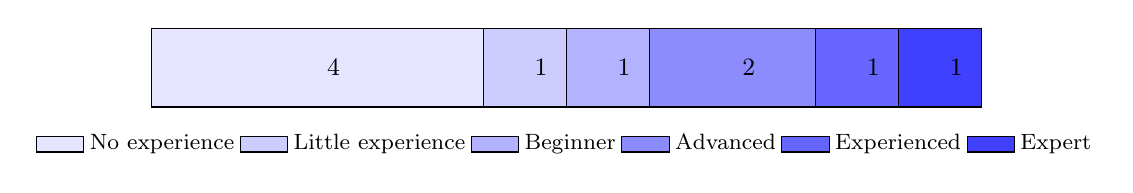
\begin{tikzpicture}
    \pgfplotsset{testbar/.style={
        xbar stacked,
        area style,
        width=\textwidth,
        height=2cm,
        xmajorgrids = false,
        xmin=0, xmax=10, % Adjust max to sum of all values
        ytick=\empty,
        xtick=\empty,
        bar width=15mm,
        y=8mm,
        enlarge y limits={abs=0.625},
        nodes near coords,
        every node near coord/.append style={rotate=0, anchor=west, font=\small}
    }}

    \begin{axis}[testbar,
        legend style={at={(0.5,-0.2)}, anchor=north, legend columns=-1, font=\footnotesize, draw=none}]
        \addplot[fill=blue!10] coordinates{(4,0)};
        \addplot[fill=blue!20] coordinates{(1,0)};
        \addplot[fill=blue!30] coordinates{(1,0)};
        \addplot[fill=blue!45] coordinates{(2,0)};
        \addplot[fill=blue!60] coordinates{(1,0)};
        \addplot[fill=blue!75] coordinates{(1,0)};

        \legend{No experience, Little experience, Beginner, Advanced, Experienced, Expert}
    \end{axis}
  \end{tikzpicture}
  \caption{Participant Experience Levels}
  \label{fig:study:experience}  
\end{figure}

Four of the participants have backgrounds in filmmaking, including directors, camera operators, and post-production specialists.
The remaining six are software developers and researchers, selected for their expertise with NeRF or human-computer interaction.

\section{Tasks Based Usability Test}
\label{sec:study:tasks}

The usability test was conducted in a controlled environment, where participants were asked to complete several tasks with the prototype.
These tasks were designed to cover a range of functionalities and features of the prototype, representing a typical workflow for creating NeRF models.
The tasks included:

\begin{enumerate}
  \item Creating a new project.
  \item Uploading a prepared video file.
  \item Pre-processing the uploaded file to prepare it for training.
  \item Switching to an existing project with pre-processed data.
  \item Starting a NeRF training.
  \item Creating a camera path in the viewer.
  \item Exporting a video.
\end{enumerate}

To maintain an appropriate time frame, none of the tasks required completion of a training process, and pre-processed data and pre-trained models were provided.
On average, participants took 30 minutes to complete the tasks.

Participants were passively observed while working on their tasks to identify any problems or operational errors they encountered and to determine their overall performance.
Additionally, the screen was recorded to capture participants' interactions with the prototype, allowing for a more detailed analysis of their behavior later on.

\section{User Experience Questionnaire}
\label{sec:study:ueq}

After completing their tasks, participants were asked to fill out the User Experience Questionnaire (UEQ) \cite{laugwitz_construction_2008}, a standardized tool for assessing user experience.
The UEQ was done immediately after the tasks to capture participants' immediate impressions while the experience was still fresh in their minds, and before any influence from the follow-up interview.
Due to an oversight, the UEQ was not administered before the tasks for the studies conducted remotely.

The UEQ measures user experience across six dimensions:

\begin{itemize}
  \item \textbf{Attractiveness} - the overall impression of the product.
  \item \textbf{Perspicuity} - the clarity and understandability of the product.
  \item \textbf{Efficiency} - the perceived effort required to use the product.
  \item \textbf{Dependability} - the perceived reliability and trustworthiness of the product.
  \item \textbf{Novelty} - the perceived originality and innovation of the product.
  \item \textbf{Stimulation} - the perceived level of excitement and engagement with the product.
\end{itemize}

This tool covers both classical usability goals (Efficiency, Perspicuity, Dependability) and user experience qualities (Novelty, Stimulation), with Attractiveness serving as a valence dimension not directly related to usability or user experience.

The questionnaire consists of 26 items, each represented by two terms of opposite meaning, with the order of the terms randomized for each item to avoid bias.
Participants rate each item on a 7-point scale from -3 to +3, with 0 representing a neutral response.
An example of the scale is as follows:

\begin{center}
  \emph{boring} \quad o o o o o o o \quad \emph{exciting}
\end{center}

Participants filled out the questionnaire digitally using a web-based survey tool \cite{noauthor_sosci_nodate}, which also included additional questions to gather demographic information and capture prior experience with NeRF and other 3D modeling tools.

\section{Follow-up Interview}
\label{sec:study:interview}

After completing the usability test, participants engaged in a short follow-up interview to provide more detailed feedback on their experience with the prototype.
These interviews were semi-structured, following a predefined set of questions with room for participants to share their own thoughts and suggestions.
Questions focused on participants' overall impressions of the prototype, usability challenges they encountered, and suggestions for improvement.
The interview template is included in Appendix \ref{sec:appendix:questionnaire}.

\section{Data Analysis}
\label{sec:study:analysis}

Both the video recordings of the usability test and the audio recordings of the follow-up interviews were analyzed to identify common themes and patterns in participant feedback.
Videos were coded to highlight usability issues or challenges encountered during tasks, while interview transcripts were coded to extract detailed feedback and suggestions.

The UEQ data was analyzed using the standard procedure provided by the questionnaire's authors, which includes a spreadsheet tool that calculates all necessary values and visualizes the results.

In summary, this user study and evaluation was pivotal in validating the effectiveness of the NeRF interface prototype, uncovering valuable insights into its usability, and identifying opportunities for further refinement.
The mixed-methods approach ensured a comprehensive assessment, capturing both tangible aspects of interface interaction and the subjective experiences of users, providing a solid foundation for subsequent development stages.
